\chapter{TLAV - Thinking Like a Vertex}

MapReduce + HDFS is a solution for many BigData problems, as it allows for processing large amounts of data in a distributed manner. However, it is not the best solution for all use cases, as it has some limitations, such as high latency and lack of real-time processing capabilities.

\note{Recall that HDFS is a distributed file system that allows for storing large amounts of data across multiple machines.}

\section{Spark SQL}
Spark SQL allows to execute SQL queries, which are translated into Spark jobs (more precisely as \textit{actions} and \textit{transformations}). It is built on top of the Spark Core, and provides a more user-friendly interface for working with data.
The result is yielded as a DataFrame, which is a distributed collection of data organized into named columns, on which we may execute various operations by means of a high-level SQL \verb|spark.sql("SELECT * FROM people")| API.

\subsection{Structured Streaming}
Structured Streaming is a scalable and fault-tolerant stream processing engine built on the Spark SQL engine.


Streaming computation represented in the same way of a batch computation on static data.
The Spark SQL engine will take care of running it incrementally and continuously and updating the final result as streaming data continues to arrive.

The system \ul{ensures \textit{end-to-end exactly-once fault-tolerance} guarantees} through
checkpointing and \textbf{Write-Ahead Logs}.

When we say ``exactly-once semantics'' we mean that each incoming event affects the final results exactly once. Even in case of a machine or software failure, there’s no duplicate data and no data that goes unprocessed.

\begin{paracol}{2}
   The key idea in structured streaming is to treat a live stream as if it were a table that is being continuously appended. This allows for writing SQL queries that process the data in real-time, and to get the results as soon as new data arrives.
   
   Consider the input data stream as the ``Input Table''. Every data item that is arriving on the stream is like a new row being appended to the Input Table.

   A query on the input will generate the ``Result Table''. Every trigger interval, new rows get appended to the Input Table, which eventually updates the Result Table. Whenever the result table gets updated, we would want to write the changed result rows to an external sink
\switchcolumn
   \begin{figure}[htbp]
      \centering
      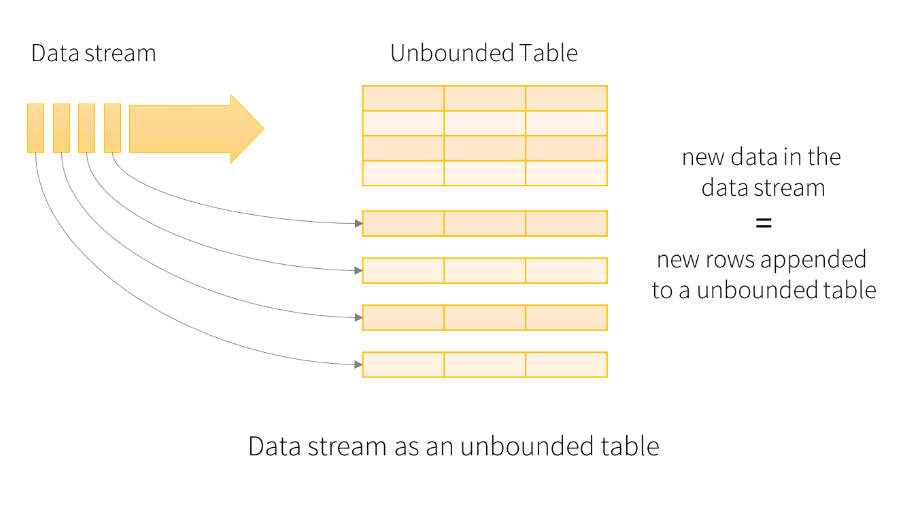
\includegraphics{images/18/sparktable.png}
      \caption{Structured Streaming schema}
      \label{fig:18/sparktable}
   \end{figure}

\end{paracol}

\framedt{Output mode}{
\begin{itemize}
	\item \textbf{Complete} Mode - The entire updated Result Table will be written to the external storage. It is up to the storage connector to decide how to handle writing of the entire table.
	\item \textbf{Append} Mode - Only the new rows appended in the Result Table since the last trigger will be written to the external storage. This is applicable only on the queries where existing rows in the Result Table are not expected to change.
	\item \textbf{Update} Mode - Only the rows that were updated in the Result Table since the last trigger will be written to the external storage.
      \begin{itemize}
      	\item Note that this is different from the Complete Mode in that this mode only outputs the rows that have changed since the last trigger.
      	\item If the query doesn’t contain aggregations, it will be equivalent to Append mode
      \end{itemize}
\end{itemize}
}

\begin{figure}[htbp]
   \centering
   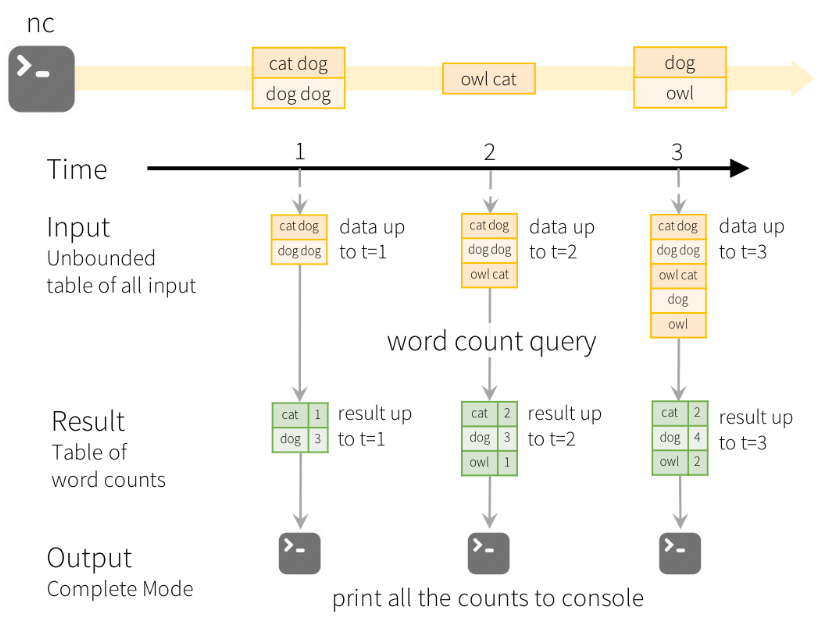
\includegraphics{images/18/sparkexample.png}
   \caption{Spark query output example}
   \label{fig:18/sparkexample}
\end{figure}

Note that Structured Streaming does not materialize the entire table.
It reads the latest available data from the streaming data source, processes it incrementally to update the result, and then discards the source data.
It only keeps around the minimal intermediate state data as required to update the result.

\section{Working on Graphs}
Graphs are a powerful data structure that can be used to represent complex relationships between entities.
A graph is made up of vertices (also called nodes) and edges (also called links).

We may use MapReduce to process graphs, but it is not the most efficient way to do so, as it requires multiple passes over the data, and it is not well-suited for iterative algorithms.
MapReduce forces to think in terms of a linear sequence of operations, which does not fit well with the nature of graph algorithms, which are often iterative and require multiple passes over the data.

\subsection{GraphX}

GraphX is a distributed graph processing framework built on top of Apache Spark. It provides a set of APIs for working with graphs, and allows for the execution of graph algorithms in a distributed manner.
GraphX represents graphs as a combination of two RDDs: one for the vertices and one for the edges.
This allows for efficient processing of large graphs, as the data can be partitioned and distributed across multiple machines.

GraphX exploits the concept of TLAV - Think Like a Vertex, which is a programming model for graph processing that allows the user to define a function that is executed on each vertex of the graph.

\subsubsection{TLAV - Think Like a Vertex}
In TLAV, the programming logic is organized around vertices, which are the primary
units of computation.

Each vertex maintains its state (i.e., its label and attribute) and can send messages
to its neighbouring vertices based on its state and the state of its neighbours.
The messages are then received by the neighbouring vertices, which can update
their state accordingly.

TLAV is a powerful abstraction that can be used to express a wide range of graph
algorithms in a concise and efficient manner. By thinking like a vertex, you can
design efficient and scalable graph algorithms that can process large-scale graphs
in a distributed environment.

\subsubsection{Actor Model and TLAV}

In GraphX, the actor model is used to represent vertices in a graph and to perform distributed graph processing.

Each vertex is represented as an actor, which communicates with other actors by exchanging messages. By using the actor model, GraphX provides a programming model for distributed graph processing that is based on vertex-centric computations.

In GraphX, the computation proceeds in a series of supersteps, where each superstep consists of message passing and vertex computations. In each superstep, each vertex receives messages from its neighbours and updates its state based on those messages. After each superstep, the vertices exchange messages and the computation proceeds to the next superstep.